Time-series prediction of the neural model relies on the input history of equally distributed samples.
The LSTM model is a recurrent neural network that designs to solve the vanishing gradient problem by remembering/preserving the long dependencies~\cite{rasifaghihi_predictive_2020}.
The cells inside the model act as memory units to preserve the dependence.
Therefore, the output is closely dependant on the previously input samples.
Unlike the normal RNN and the more modern version - GRU, LSTM has a more complicated structure constructed from several logical gates~\cite{LSTM_Hochreiter1997}.
It is the most widely used type of model.
Figure~\ref{fig:LSTM-cell2} provides summary of the cell logic.
It utilises 3 gates: forget $f_t$, input $i_t$ and output $o_t$, as per equation~\ref{eq:LSTM-gates2}.
The decisions based around sigmoid $\sigma$ function~\ref{eq:sigmoid2}.
With default $tanh$ as activation function, equation~\ref{eq:LSTM-output2} describes the procedure for cell state update and further propogation.
$h_t$ and $c_t$ represent memory cell output and the cell state at timestamp $t$.

%
%
\begin{equation}
    \sigma(x) = \frac{1}{1+e^{-x}}
    \label{eq:sigmoid2}
\end{equation}
\begin{figure}[ht]%[htbp]
    \centering
    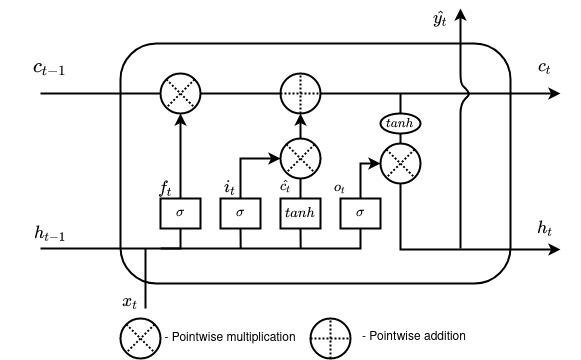
\includegraphics[width=0.7\linewidth]{II_Body/LSTM/images/LSTM.jpg}
    \caption{Long Short-Term Memory Cell}
    \label{fig:LSTM-cell2}
\end{figure}
\begin{equation}
    \begin{split}
        f_t &= \sigma \left(W_f \left[h_{t-1}, x_t \right] + b_f \right) \\
        i_t &= \sigma \left(W_i \left[h_{t-1}, x_t \right] + b_i \right) \\
        o_t &= \sigma \left(W_o \left[h_{t-1}, x_t \right] + b_o \right) \\    
    \end{split}
    \label{eq:LSTM-gates2}
\end{equation}
\begin{equation}
    \begin{split}
        \hat{c_t} &= tanh \left(W_c \left[h_{t-1}, x_t \right] + b_c \right) \\
              c_t &= f_t c_{t-1}+i_t \hat{c_t} \\
              h_t &= o_t*tanh \left(c_t \right)
    \end{split}
    \label{eq:LSTM-output2}
\end{equation}
The LSTM model has been used widely in stock-price prediction or weather forecasting.
Unlike State of Charge estimation, which commonly uses $V$, $I$ and $T$ as inputs, those methods utilise the output feature as an input to the subsequent prediction to propagate results further and calculate the time before a critical event occurrence.
Besides, methods like temperature prediction a weak ahead are not limited by lacking output data.
Contrarily, a True State of Charge of a battery cannot be determined and verified against previously made predictions without using some additional battery modelling techniques.
%%%%%%%%%%%
%Unlike the charge estimation, which can only output a single value based on a history of samples, they are not limited to... Therefore does not require the output as input since the truth will become known in due time.

%
%
The best way to utilise the performance of the stateless LSTM model is through training with a data windowing technique.
The NN model will receive a fixed set of equally distributed time samples at each time prediction.
Every next forecast will shift the time window by a constant step $s$, until all possible combinations of time slices went through the model.
That approach referred to as a stateless model, which sees dependencies over input samples only, rather than preserving for every received input.
It also allows the order of the windows to be shuffled to avoid overfitting since no dropout technique is used in model initialisation.
As a result, a NN model will learn dependency between a fixed amount of equally distributed time samples $n$ and yet independent from the order of the inputs.
Figure~\ref{fig:Windowing} demonstrates how the input dataset constructed and ordered into a 3-dimensional dataset.
Due to the size of the windows of 500 samples, which equivalent to 5 minutes of a discharge process, no batching mechanism has been used to reduce computational load and avoid 4-dimensional matrix management.


%
%
The mean and standard deviation has normalised all data to speed up the training process.
The normalisation constant from training input samples must be used for validation and testing sets to ensure the right trends.
The percentage of the state of charge will be narrowed between 0 and 1 to represent the percentage charge.
The Table~\ref{tab:params} highlights parameters required to define the initial model.
Use of a $\sigma$ function as an output justified by the charge normalisation between 0 and 1.
\begin{table}[ht]
    \centering
    \caption{Model structure and parameters}
    \label{tab:params}
    \begin{tabular}{ p{3.0cm} p{3.5cm} p{2.5cm}   }
        \hline
        Input     & $shape= \left( 1,500,4 \right)$ & $batch=1 $  \\
        \hline
        LSTM      & $activation= 'tanh'$ & $units=510$  \\
        \hline
        Dropout   & $0.0$ &   \\
        \hline
        Output    & $activation= \sigma\left(1\right)$ &   \\
        \hline
    \end{tabular}
\end{table}

%
%
Data were taken from CALCE University, cycling temperatures of 20,25,30 degrees over three driving profiles.
The FUDS driving scheduler acts as a training set, then the other two DST and US06 for testing.
The choice of validation sets was due to differences in the current consumption.
If DST has a constant variation of the current amps over time, the US06 uses an aggressive mechanism, similar to the FUDS.
The ability to accurately capture both driving mechanisms with minor error acts as a validation mechanism and justifies the value of the technique.

%
%
The optimisation algorithm for the fitting process has been defined by Adam, Algorithm~\ref{alg:Adam}, with the following hyperparameters, Table~\ref{tab:newM-params}. \\
%\textcolor{red}{Try to use Robust Adam instead first, because why the hell not since I lost one month of my life to implement that cursed algorithm from Javids miss-typed notes. Complete this section with details as per Gareth Javid implementation if RoAdam will be able to produce a faster fitting.}
\begin{table}[htbp]
    \centering
    \caption{Optimiser specific hyperparameters}
    \label{tab:newM-params}
    \begin{tabular}{ p{1.5cm} p{1.5cm} p{1.5cm} p{1.5cm}  }
        \hline
        $\alpha$ & $\beta_1 $ & $\beta_2$ & $\epsilon$ \\
        \hline
        $0.001$ & $0.9$ & $0.999$ & $10^{-8}$ \\% 0.0000001
        \hline
    \end{tabular}
\end{table}